%	PACKAGES AND OTHER DOCUMENT CONFIGURATIONS

\documentclass[11pt, a4paper]{article} % 10pt font size (11 and 12 also possible), A4 paper (letterpaper for US letter) and two column layout (remove for one column) Use additional titlepage argument to generate this
%\documentclass[12pt, a4paper,twocolumn,titlepage]{article}

%%%%%%%%%%%%%%%%%%%%%%%%%%%%%%%%%%%%%%%%%
% Wenneker Article
% Structure Specification File
% Version 1.0 (28/2/17)
%
% This file originates from:
% http://www.LaTeXTemplates.com
%
% Authors:
% Frits Wenneker
% Vel (vel@LaTeXTemplates.com)
%
% License:
% CC BY-NC-SA 3.0 (http://creativecommons.org/licenses/by-nc-sa/3.0/)
%
%%%%%%%%%%%%%%%%%%%%%%%%%%%%%%%%%%%%%%%%%

%----------------------------------------------------------------------------------------
%	PACKAGES AND OTHER DOCUMENT CONFIGURATIONS
%----------------------------------------------------------------------------------------

\usepackage[english]{babel} % English language hyphenation

\usepackage{microtype} % Better typography

\usepackage{verbatim} % Allows mulitline commenting

\usepackage{amsmath,amsfonts,amsthm} % Math packages for equations

\usepackage[svgnames]{xcolor} % Enabling colors by their 'svgnames'

\usepackage[hang, small, labelfont=bf, up, textfont=it]{caption} % Custom captions under/above tables and figures

\usepackage{subcaption}

\usepackage{booktabs} % Horizontal rules in tables

\usepackage{lastpage} % Used to determine the number of pages in the document (for "Page X of Total")

\usepackage{graphicx} % Required for adding images

\usepackage{enumitem} % Required for customising lists
\setlist{noitemsep} % Remove spacing between bullet/numbered list elements

\usepackage{sectsty} % Enables custom section titles
\allsectionsfont{\usefont{OT1}{phv}{b}{n}} % Change the font of all section commands (Helvetica)

\usepackage{siunitx}

%----------------------------------------------------------------------------------------
%	MARGINS AND SPACING
%----------------------------------------------------------------------------------------

\usepackage{geometry} % Required for adjusting page dimensions

\geometry{
	top=1cm, % Top margin
	bottom=1.5cm, % Bottom margin
	left=2cm, % Left margin
	right=2cm, % Right margin
	includehead, % Include space for a header
	includefoot, % Include space for a footer
	%showframe, % Uncomment to show how the type block is set on the page
}

\setlength{\columnsep}{7mm} % Column separation width

%----------------------------------------------------------------------------------------
%	FONTS
%----------------------------------------------------------------------------------------

\usepackage[T1]{fontenc} % Output font encoding for international characters
\usepackage[utf8]{inputenc} % Required for inputting international characters

\usepackage{XCharter} % Use the XCharter font

%----------------------------------------------------------------------------------------
%	HEADERS AND FOOTERS
%----------------------------------------------------------------------------------------

\usepackage{fancyhdr} % Needed to define custom headers/footers
\pagestyle{fancy} % Enables the custom headers/footers

\renewcommand{\headrulewidth}{0.0pt} % No header rule
\renewcommand{\footrulewidth}{0.4pt} % Thin footer rule

\renewcommand{\sectionmark}[1]{\markboth{#1}{}} % Removes the section number from the header when \leftmark is used

%\nouppercase\leftmark % Add this to one of the lines below if you want a section title in the header/footer

% Headers
\lhead{} % Left header
\chead{\textit{\thetitle}} % Center header - currently printing the article title
\rhead{} % Right header

% Footers
\lfoot{} % Left footer
\cfoot{} % Center footer
\rfoot{\footnotesize Page \thepage\ of \pageref{LastPage}} % Right footer, "Page 1 of 2"

\fancypagestyle{firstpage}{ % Page style for the first page with the title
	\fancyhf{}
	\renewcommand{\footrulewidth}{0pt} % Suppress footer rule
}

%----------------------------------------------------------------------------------------
%	TITLE SECTION
%----------------------------------------------------------------------------------------

\newcommand{\authorstyle}[1]{{\large\usefont{OT1}{phv}{b}{n}\color{NavyBlue}#1}} % Authors style (Helvetica)

\newcommand{\institution}[1]{{\footnotesize\usefont{OT1}{phv}{m}{sl}\color{Black}#1}} % Institutions style (Helvetica)

\usepackage{titling} % Allows custom title configuration

\newcommand{\HorRule}{\color{SteelBlue}\rule{\linewidth}{1pt}} % Defines the gold horizontal rule around the title

\pretitle{
	\vspace{-30pt} % Move the entire title section up
	\HorRule\vspace{10pt} % Horizontal rule before the title
	\fontsize{32}{36}\usefont{OT1}{phv}{b}{n}\selectfont % Helvetica
	\color{Navy} % Text colour for the title and author(s)
}

\posttitle{\par\vskip 15pt} % Whitespace under the title

\preauthor{} % Anything that will appear before \author is printed

\postauthor{ % Anything that will appear after \author is printed
	\vspace{10pt} % Space before the rule
	\par\HorRule % Horizontal rule after the title
	\vspace{20pt} % Space after the title section
}

%----------------------------------------------------------------------------------------
%	ABSTRACT
%----------------------------------------------------------------------------------------

\usepackage{lettrine} % Package to accentuate the first letter of the text (lettrine)
\usepackage{fix-cm}	% Fixes the height of the lettrine

\newcommand{\initial}[1]{ % Defines the command and style for the lettrine
	\lettrine[lines=3,findent=4pt,nindent=0pt]{% Lettrine takes up 3 lines, the text to the right of it is indented 4pt and further indenting of lines 2+ is stopped
		\color{NavyBlue}% Lettrine colour gold DarkGoldenRod
		{#1}% The letter
	}{}%
}

\usepackage{xstring} % Required for string manipulation

\newcommand{\lettrineabstract}[1]{
	\StrLeft{#1}{1}[\firstletter] % Capture the first letter of the abstract for the lettrine
	\initial{\firstletter}\textbf{\StrGobbleLeft{#1}{1}} % Print the abstract with the first letter as a lettrine and the rest in bold
}

%	BIBLIOGRAPHY

\usepackage[backend=biber,style=phys,natbib=true,doi=false]{biblatex} 
%Can equally use numeric citation style without extra phys packaging (but doesn't change capitalisation), or authoryear for alphabetical listing without the codes (resembles APA)

%\addbibresource{references.bib} % The filename of the bibliography

\usepackage[autostyle=true]{csquotes} % Required to generate language-dependent quotes in the bibliography

%    APPENDICES

\usepackage[title]{appendix} %in appendix


 % Specifies the document structure and loads requires packages
\graphicspath{{"/Users/kit gallagher/Documents/Research Review/Report/Figures"}}
\newcommand*{\subscript}[1]{\ensuremath{_\textrm{{\scriptsize #1}}}}

%	ARTICLE INFORMATION

\title{Simulating Liquid Crystals}

%\author{
	%\authorstyle{Christopher Gallagher}}
\author{\authorstyle{Kit Gallagher} 
	%\institution{University of Cambridge \\
	\institution{Supervisors: Prof Erika Eiser, Mr Jiaming Yu}}
% Example of a one line author/institution relationship
%\author{\newauthor{John Marston} \newinstitution{Universidad Nacional Autónoma de México, Mexico City, Mexico}}

\date{\today} % Add a date here if you would like one to appear underneath the title block, use \today for the current date, leave empty for no date
\usepackage[english]{babel}
\usepackage{tabularx}
%\renewcommand{\thefootnote}{\roman{footnote}}  %use roman lettering for footnotes instead
%\usepackage[backend=biber,doi=false]{biblatex}
\addbibresource{reportreferences.bib}
%\AtBeginBibliography{\small}
%----------------------------------------------------------------------------------------
\begin{document}
	
%Your project should contain the following statement on the first page of the project: Except where specific reference is made to the work of others, this work is original and has not been already submitted either wholly or in part to satisfy any degree requirement at this or any other university.	A link to your on-line notebook should also be added to the first page of your report before uploading the project.

\maketitle % Print the title

\thispagestyle{firstpage} % Apply the page style for the first page (no headers and footers)

%	ABSTRACT

\lettrineabstract{The specificity of DNA base-pair interactions gives considerable functional control in the design of anisotropic nano-particles, enabling the formation of liquid crystal phases. This project aims to study the liquid phase behaviour of such non-conventional liquid crystal molecules, with a particular focus on the novel `nunchuck' structure - two rigid rods connected via a flexible linker. The Eiser Group have previously considered intra-molecular interaction potentials at the single-nucleotide level for a single DNA nanoparticle, and I am now implementing these potentials in larger, more coarse-grained models of multiple nanoparticles, through open-source software LAMMPS (Large-scale Atomic/Molecular Massively Parallel Simulator). Such systems are expected to form smectic (layered) phases at high volume fractions. THIS WILL BE EDITED AT THE END}

\section{Introduction}
What are we studying? (brief) - introduce nunchuck particles (but not implementation)
Why are we interested? Applications of this! 
-Highlight motivations both in applications but also expanding knowledge of understudied area
% intro to entropically driven transitions

Outline of report

\section{Background}
\subsection{Liquid Crystals}
Include known phases etc - de gennes textbook gives useful milestone references 
focus on entropic phase transitions % ie https://www-nature-com.ezp.lib.cam.ac.uk/articles/332822a0

\subsection{Onsager Theory} \label{sec:OnsagerTheory}

Onsager predicted a simple model of lyotropic, entropy-driven phase transitions \cite{Onsager1949}, which will be employed in this project. Rod-like particles are modelled as thin spherocylinders with length $L$ and diamater $D$, and an excluded volume preventing overlap. The interaction potentials between molecules are neglected, and only the configurational entropy of the system considered. Qualitatively, the confinement of rods to parallel orientations (such as in the nematic phase) leads to a decrease in orientational entropy, but an increase in positional entropy (as each rod takes up less space). At sufficiently high concentrations, the positional entropy will dominate, and the system undergo a phase transition from isotropic to nematic. 

The critical volume fraction at transition is approximately $4r/L$, where $r$ is the radius of the rigid rod, and $L$ is the length (detailed of this are given in Appendix \ref{sec:OnsagerAppendix}. Crucially, this means the isotropic--nematic phase transition occurs at lower concentrations for mesogens with greater aspect ratios, and requires a minimum aspect ratio of $L/r = 4$ to occur.

It is worth noting that this result is only valid in the limit of thin spherocylinders, as Onsager's derivation neglects Virial coeffecients $B_{n}$ beyond second order in the expansion of free energy in powers of density \cite{Frenkel1987}; further discussion of this is given in Appendix \ref{sec:OnsagerAppendix}.
%last sentence could go into appendix

\subsection{Order Parameter}
%smectic order given by frenkel https://pubs.acs.org/doi/pdf/10.1021/j100322a042
%can also use https://www.tandfonline.com/doi/full/10.1080/00268976.2018.1471231

The degree of order in a liquid crystal phase is characterised by an order parameter, chosen such that it is non zero in the ordered phase but vanishes in the isotropic phase. A familiar example of this is the magnetisation $\textbf{M}$ of a ferromagnet; when raised above a critical temperature, the magnetisation vanishes as the ferromagnet undergoes a phase transition. While the choice of order parameter for the nematic phase transition is less intuitive than this, it relies on the formation of genuine long-range orientational order. We may therefore define the angle ($\theta$) between each molecule's axis and the system director, and traditionally let the order parameter S be given by:

\begin{equation}
S_{n} = \left\langle P_{2}(\cos(\theta)) \right\rangle = \left\langle \frac{3}{2}\cos^{2}(\theta) - \frac{1}{2} \right\rangle 
\end{equation}

where $P_{2}$ simply denotes the second Legendre polynomial \cite{deGennes1993}. While $\langle \cos^{2}(\theta) \rangle$ would function alone as the order parameter, this has the useful property of giving unity for a perfectly aligned system, and zero for a completely random system. Further motivation for this choice is provided in Appendix \ref{sec:OrderParamTheory}.

%add description of pair-wise orientational order coeff

Similarly we will find it helpful to define a smectic order parameter $S_{s}$, to characterise the formation of one-dimensional long-range positional order. Intuitively, we expect a non-zero Fourier component of the normalised density along the director \cite{Polson1997}, and so we may write:

\begin{equation}
S_{s} = \frac{1}{N} \left\lvert \sum_{j=1}^{N} \exp \left( {\frac{2\pi}{L}i\textbf{r}_{j} \cdot \boldsymbol{\hat{n}}} \right) \right\rvert
\end{equation}

for a layers of periodicity $L$ perpendicular to the nematic director $\boldsymbol{\hat{n}}$, and where $\textbf{r}_{j}$ denotes the centre of mass position of the $j$th molecule \cite{Dussi2018}.

\subsection{Previous Computational Work} \label{sec:PrevWork}

\section{Methods}
As introduced in Section \ref{sec:PrevWork}, all molecular dynamics simulations were completed in LAMMPS. LAMMPS (Large-scale Atomic/Molecular Massively Parallel Simulator) is a medium coarse-grained, classical molecular dynamics code developed to replicate  solid-state materials and soft matter mesoscopic systems \cite{Plimpton1995, LAMMPS}.


%Can expand on this if needs be, from rapaport

\subsection{Simulation Molecules} \label{sec:SimMolecules}
As introduced in Section \textbf{X}, we are considering `nunchuck' molecules formed of two rigid rods connected by a flexible linker, as depicted in Figure \ref{fig:nunchuck_analogy}. However, as the interaction potential of an anisotropic particle is rather complex, it is computationally simpler to consider each molecule as a system of connected spheres, each with a separate isotropic interaction potential (detailed further in Section \ref{pair_potential}).

This is visualised in Figure \ref{fig:nunchuck_implementation}, for rigid arms of aspect ratio 7. The ss-DNA is represented by a further sphere in the centre of the molecule, coloured differently in red to highlight its differing mechanical properties. It has a modified bond angle, so the molecule is bent around this element, and reduced bond rigidity so the particle may also stretch about this point. We also consider a simplified system of rigid rods with no modifications on the central atom, to verify the analysis methods against known results.

\begin{figure}[ht]
	\hfill  %NOT SURE ABOUT THIS!
	\begin{subfigure}{.4\textwidth}
		\centering
		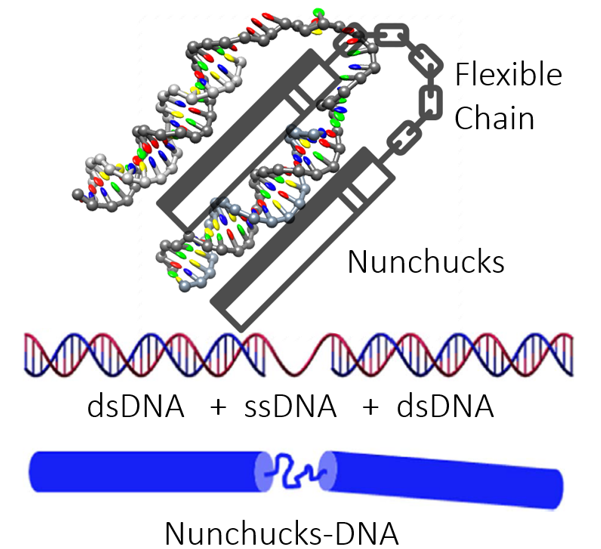
\includegraphics[width=\linewidth]{Figures/nunchucks_artist}  
		\caption{Coarse-grained Model}
		\label{fig:nunchuck_analogy}
	\end{subfigure}
	\hfill %% useful if width of each figure is less the .5\textwidth
	\begin{subfigure}{.4\textwidth}
		\centering
		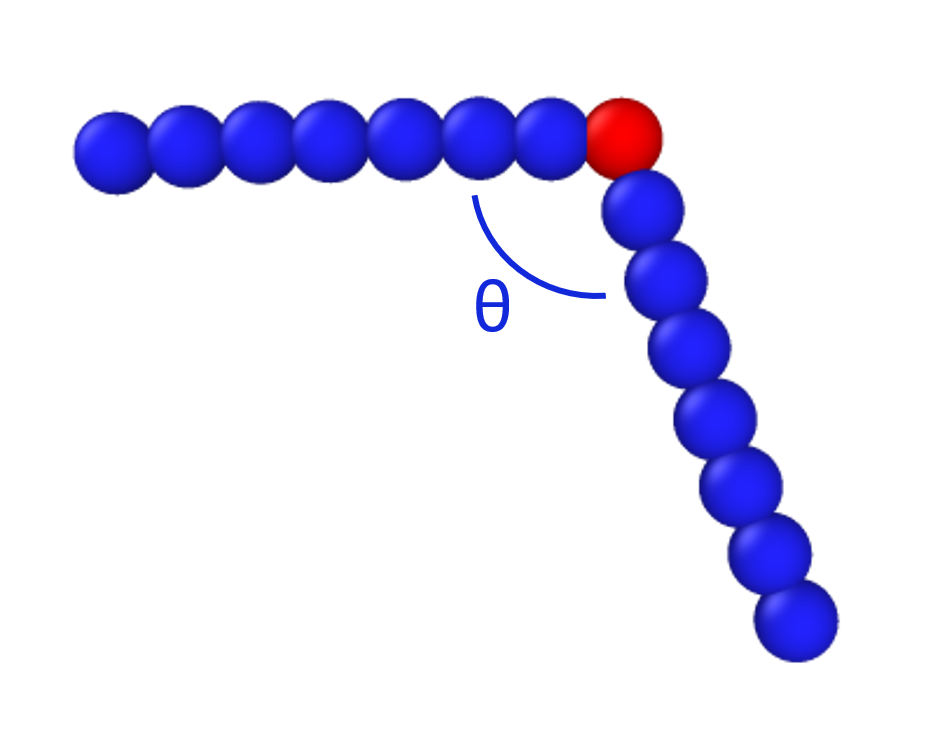
\includegraphics[width=\linewidth]{Figures/nunchuck_profile_coloured}  
		\caption{LAMMPS Implementation}
		\label{fig:nunchuck_implementation}
	\end{subfigure}
	\caption{Depiction analogy between the DNA mesogen and the nunchucks. Note the appearance of the flexible ss-DNA linker between the rigid ds-DNA rods, and the implementation within LAMMPS on the right. The central red sphere, representing the ss-DNA, is given modified bond properties to replicate the nunchuck's flexibility. Figure (a) created by Jiaming Yu (Eiser Group, Cambridge).}
	\label{fig:nunchucks_visual}
	\hfill
\end{figure}

A system of natural units was used in simulations, and replicated in our results here. Based on the Lennard-Jones potential, the cut-off length and characteristic energy are both set to unity. The simulation timescale is then fixed by the choice of these values, and the mass of the simulation body. 

The physical values for a system may be considered for a specific system (in this case strands of ds-DNA) through scaling via the relevant mass, length scale and energy scale of this system. However the dimensionless simulations presented here may be generalised to any similarly-shaped mesogens; we would expect other systems to display the same behaviour over an appropriate timescale determined by their material properties \cite{Rapaport2004}.

For the nunchuck particles considered, a length scale of \SI{2}{\nano\metre} is used (corresponding to the width of ds-DNA, and hence the diameter of a simulation sphere) \cite{Arnott1972}. It is worth noting that the persistence length of DNA is around \SI{50}{\nano\metre} \cite{Garcia2007}, so the approximation of perfect rigidity is valid for all rods considered here (maximum length \SI{30}{\nano\metre}). Using the standard value of \SI{0.33}{\nano\metre} \cite{Langridge1960} for the average length of a base pair, each sphere corresponds to a sequence of six base pairs. This gives the mass of each sphere as \SI{6.5e-24}{\kilogram}, based on an average formula mass per base pair of \SI{650}{\dalton} \cite{Duewer2018}). 

We may also define the characteristic energy scale; this is formally the depth of the potential well in the full Lennard-Jones potential, but the thermal energy serves as a common approximation \cite{Pan2010} in agreement with experimental data \cite{Wang2002}. Using these values, we find that the characteristic timescale for this system is \SI{79}{\pico\second}. In this context, the simulation timestep would be \SI{0.4}{\pico\second}, and typical simulation of \num{20e6} steps had a total duration of \SI{7.9}{\micro\second}. For \num{1000} particles, this took approximately $8$ hours to run on a standard laptop CPU. %check these



\subsection{Simulation Structure} %was? is? check your tense here!
All simulations in this report were conducted a system of 1000 particles, with a time step of $0.005\tau$, (where $\tau$ is the characteristic time), unless otherwise stated. The system was initially configured in a dilute, isotropic state; a non-trivial process for large numbers of mesogens as molecules must be placed randomly without overlap, to prevent any initial order affecting the formation of ordered phases. I am grateful to Iria Pantazi for writing a python script to automate this process for dilute rigid rod systems, and a generalised version of this is available in the supplementary material. Alternatively, simulations were also initiated from a perfectly ordered square crystalline phase, with all molecules aligned along a common axis. The choice of this axis is arbitrary, as the system is invariant under global rotation \cite{Nos1983}, but is taken to be directed along the y-axis for clarity. Care was taken to ensure molecules did not overlap, and the system was stable in this ordered phase.
%MAYBE INCLUDE CODE IN SUPP MATERIAL?? THINK ABOUT THIS!

All simulations are conducted within an oblong box defined by the Cartesian axes, with periodic boundary conditions used to eliminate surface effects and replicate conditions in the bulk phase \cite{Frenkel2002}. The aspect ratio of this box may be varied, to support phase formation in anisotropic systems, as discussed in Section \textbf{X}. An isenthalpic ensemble was used (where pressure is fixed) to vary the size of the simulation region (either contracting or expanding), allowing sampling of different volume fractions from the same initial configuration. The microcanonical ensemble, where both the system volume and energy are conserved, was then used to allow the system to reach thermodynamic equilibrium. Time integration was evaluated using the Nose-Hoover thermostat \cite{Nos1984, Hoover1985} natively implemented in LAMMPS \cite{Shinoda2004}, typically with a damping time of $\tau$.

A typical simulation consists of multiple stages, alternating between these two ensembles to sample the system properties at a range of volume fractions. Approximately \num{2e4} steps are simulated when varying the simulation volume (depending on the resolution of volume fraction sampling), followed by \num{2e6} to allow the system to reach equilibrium in each stage. The output of thermodynamic variables, as well as particle positions, at the end of each stage allows for subsequent calculation of the order parameter at equilibrium. This data was also retrieved at regular intervals during each simulation stage, to track the time evolution of the system.

To ensure stability of the system, a Langevin thermostat \cite{Schneider1978} was also used throughout, and energy conservation was verified over a range of timescales. The damping for all thermostats is equal to the characteristic timescale of the simulation (i.e. unity in natural units).



\subsection{Intermolecular Potential} \label{pair_potential}
A shifted, cut-off Lennard-Jones potential was chosen to represent pair-wise interactions between molecules. While the Lennard-Jones potential \cite{Jones1924a, Jones1924b} has long been the natural choice for molecular dynamics simulations \cite{Stephan2019}, its infinite range introduces computational complexity as interactions between all pairs of particles must be considered. It is therefore increasingly common to use a cut-off version, whereby the potential is set to zero beyond a `cut-off' radius, and here we chose to neglect the entire attractive tail. As well as simplifying the calculations required, this also allows our results to be generalised to any mesogens without attractive inter-molecular forces (that typically favour ordered-phase formation), as any phase transitions observed here must be purely entropically driven. This is commonly known as a soft-core model, where particle overlap is suppressed via this repulsive potential rather than any excluded volume interactions, and is computationally much less demanding \cite{Paolini1993, Hughes2008}.
%can cite frenkel on entropically drive transitions if req

However, this cut-off may cause unphysical behaviour if the potential does not tend to zero smoothly at this point. This is remedied by the addition of a constant term, described in the full form of the pair-wise potential $U_{ij}$ in (\ref{lj_cut}):

\begin{equation} \label{lj_cut}
U_{ij} = 4\epsilon \left[ \left( \frac{\sigma}{r_{ij}} \right) ^{12} - \left( \frac{\sigma}{r_{ij}} \right) ^{6}	\right] + \epsilon \qquad	 r_{ij} < r_{c} = 2^{1/6} \sigma
\end{equation}

Here $\sigma$ and $\epsilon$ are the relevant length and energy scales of the system, formally corresponding to the particle separation at which the $U_{ij} = 0$, and the depth of the potential well. It is worth noting that the effects of this truncation and shift on the overall thermodynamic quantities are well documented \cite{Stephan2020, Shaul2010}, and changes in lyotropic properties are negligible in 3D bulk liquids with a conserved particle number \cite{Smit1991}. 

 
\subsection{Analysis}
The visualisation freeware Ovito \cite{Ovito} has been employed to animate the molecule motion over the simulation period, and was used to generate all molecular images presented here. Thermodynamic variables, such as internal energy and pressure, were extracted to track the system's progress towards equilibrium, and verify its stability.

The volume fraction and nematic order parameter were computed for comparison with Onsager's theorem, as detailed in Section \ref{sec:OnsagerTheory}. Calculation of the order parameter is complicated by the absence of an imposed director (ie if no electric field is applied), and we use the approach taken by Eppenga and Frenkel \cite{Eppenga1984} which is reproduced in Appendix \ref{sec:OrderParamCalc}. %or dussi 2018 or many others

Further analysis included the calculation of the smectic order parameter, and pair-wise orientational correlation coefficient, detailed in Section \textbf{X}. All scripts for data extraction and analysis were written by the author, \textit{and can be found in the supplementary material?}.



\section{Rigid Rod Simulations} \label{sec:RigidRodSims}
%Used to benchmark sys etc and demonstrate techniques to identify phase transitions.
%Detail nematic phase transition (longrun4) and validation through onsager theory
%Extend this with the longer rods which continue to confirm this theory


Initially, a system of rigid rods was used to verify the analysis methods applied in this report, in comparison with the predictions made by Onsager's theory in Section \ref{sec:OnsagerTheory}. We focus specifically on the phase transition between the isotropic and nematic phases, as this system is well studied, and these predictions have been separately verified computationally through both Monte Carlo \cite{Frenkel1984, Lee1987} and molecular dynamics simulations \cite{Allen1987, Camp1996}.
%not experimentally; long range maier-snape is better here https://pubs.acs.org/doi/pdf/10.1021/j100303a008

\subsection{Contracting Simulations}

For rigid rods with an aspect ratio $L/D = 10$, Onsager theory predicts a lyotropic phase transition will occur, with a critical volume fraction of $\phi  = 0.4$. We consider a system of \num{1000} rigid rods, formed of \num{10} sequentially connected `balls' (force-centres), and apply alternating stages of contraction (where the volume fraction is increased) and equilibration (where the volume is held constant). Each contraction stage consists of between \num{1e4} and \num{5e4} steps (chosen to identify the critical volume fraction with maximal resolution, while verifying the order parameter is approximately constant outside of this), while the equilibration stage runs for \num{2e6} steps. In this way we are able to confine the possible critical volume fraction to the range $0.39 < \phi< 0.44$, as observed in Figure \ref{fig:rr_nemorderparam}, in good agreement with Onsager's prediction of $\phi = 0.4$.

\begin{figure} [h!]
	\centering
	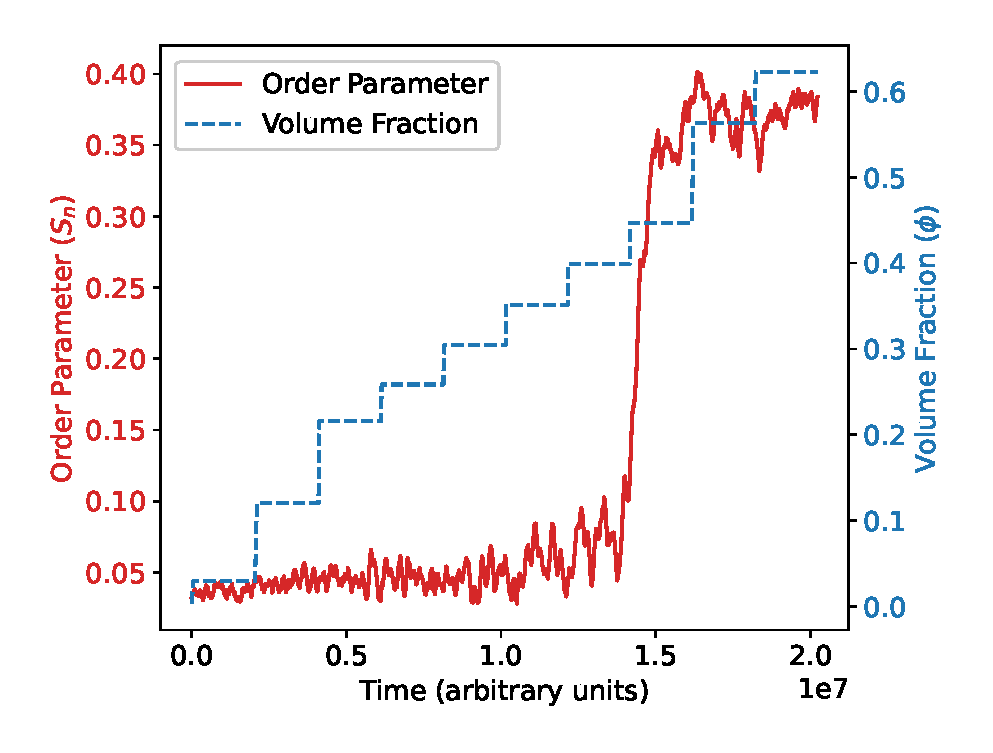
\includegraphics[width=0.7\linewidth]{Figures/rigidrod_nemorderparam}
	\caption{The evolution of the volume fraction ($\phi$) and the nematic order parameter ($S_{n}$) over the timescale of the simulation, for a system of 1000 rigid rods with aspect ratio 10. The phase transition is observed through a discrete change in the order parameter (in red), occurring after the volume fraction is increased above $0.4$. Note that the contraction steps (where volume fraction is changed) are not of equal durations, and so do not correspond to equal changes in the system volume; rather they are chosen to highlight the phase transition. The timescale of contraction is much less that the timescale of equilibration, but the changes in volume fraction are not instantaneous, despite their appearance here.}
	\label{fig:rr_nemorderparam}
\end{figure}  %C:\Users\KitG\Documents\LC_Project\Phase_Structure\Rigid_Rods2

This analysis was then repeated with longer rods, having an aspect ratio of \num{16} and a predicted critical volume fraction of $\phi  = 0.25$. Through multiple simulations, we are similarly able to verify that the critical volume fraction lies in the range $0.23 < \phi< 0.26$, in good agreement with the theory. This also provides a useful example of the characterisation of a phase transition through changes in the thermodynamic variables; Figure \ref{fig:rr_pressureevo} depicts a change in pressure during the equilibration stage of the simulation (during which volume is conserved) corresponding to the isotropic\textendash nematic phase transition.

\begin{figure} [h!]
	\centering
	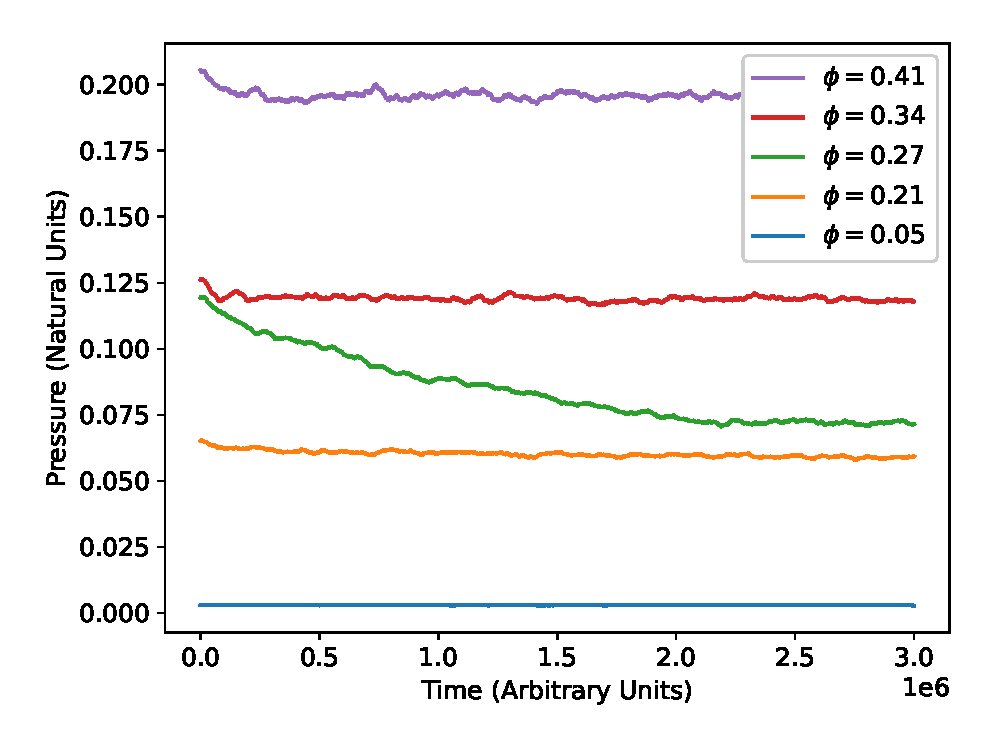
\includegraphics[width=0.7\linewidth]{Figures/rigidrod_pressureevo}
	\caption{The evolution of pressure on subsequent microcanonical ensembles (between which volume is decreased), when simulating 1000 rigid rods of aspect ratio 16. Note the extended decay in pressure for $\phi  = 0.27$, while the isotropic\textendash nematic phase transition occurs; all other stages remain at equilibrium throughout.}
	\label{fig:rr_pressureevo}
\end{figure} %C:\Users\KitG\Documents\LC_Project\Phase_Structure\Rigid_Rods2\Double_Length_Rods



\subsection{Expanding Simulations}
%Explain motivation for running simulation in reverse
%Validate location of nematic phase transition
%Introduce additional smectic phase transition (is there literature on the predicted volume fraction here?)
%explain uncertainty on nature of nematic-> smectic transition

We may also consider phase behaviour upon expansion from an perfectly ordered state, in hope of observing the same phase behaviour `in reverse'. This has two advantages; it allows us to access higher volume fractions that are not easily accessible through molecular dynamics simulations (of a reasonable duration), and also provides verification of the phase transitions previously observed. Ensuring a novel phase is in true equilibrium has long been the bane of liquid crystal simulators, however non-equilibrium effects will manifest themselves in hysteresis of the phase transition (variation in the critical volume fraction dependant on the direction of the transition), and so can be easily identified through this method.

Initially, the particle force centres are configured in a simple cubic crystalline lattice. Again equilibration stages under the microcanonical ensemble (with constant volume) are ran in alternation with an isenthalpic ensemble, however the target pressure for the Nose-Hoover thermostat is now reduced below the system pressure so that expansion occurs in these isenthalpic stages. The length of these stages is unchanged from Section \ref{sec:RigidRodSims}, however the thermostat damping is increased to $100\tau$ to ensure stability of the expansion.

\begin{figure} [h!]
	\centering
	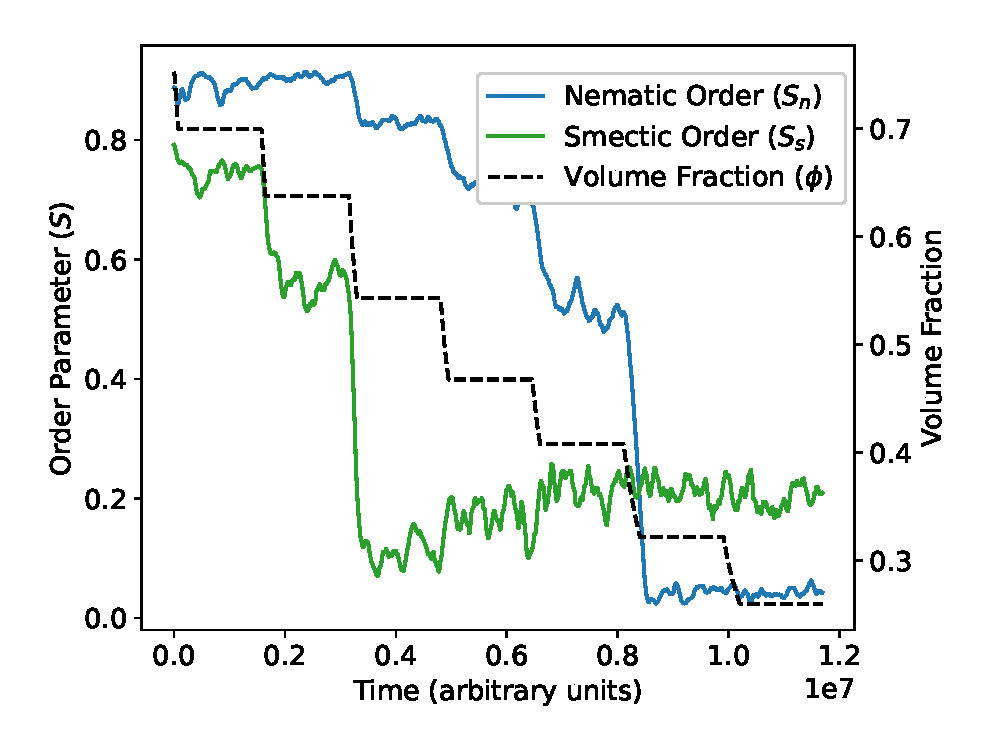
\includegraphics[width=0.7\linewidth]{Figures/rigidrod_cryorderparam}
	\caption{The evolution of the volume fraction ($\phi$) against both the nematic ($S_{n}$) and smectic ($S_{s}$) order parameters over the timescale of the simulation, for a system of 1000 rigid rods with aspect ratio 10 initiated in a crystalline phase. A continuous smectic\textendash nematic phase transition is observed (in green) at high volume fractions, followed by a discrete nematic\textendash isotropic transition (in blue), occurring after the volume fraction is decreased below $0.4$. Note that there are multiple steps in the smectic order parameter, indicating this transition occurs over a range of volume fractions.}
	\label{fig:rr_crystalorder}
\end{figure} %C:\Users\KitG\Documents\LC_Project\Phase_Structure\Rigid_Rods2\Crystalline\Full_Transition


The isotropic phase formation was observed in the region $0.38 < \phi< 0.41$, in good agreement with the results of Section \ref{sec:RigidRodSims}, and confirming this is indeed an equilibrium phase transition. 

The higher volume fractions accessed at the start of the simulation also give rise to another phase transition; forming this nematic phase from the initial ordered phase. While the system was configured in a crystalline phase, it quickly relaxes into an smectic-like phase with the one-dimensional long-range positional order. The subsequent smectic\textendash nematic transition is then observed in Figure \ref{fig:rr_crystalorder}, with a reduction in the smectic order parameter around $\phi  = 0.6$. This transition is clearly concentration-dependant (with discrete jumps in the order parameter when the volume fraction is reduced), however it occurs over a range of volume fractions and so is likely a continuous phase transition. While our evidence here is not conclusive, this is still a matter of active research and beyond the scope of this report. Theoretical \cite{Wen1987}, computational \cite{Frenkel1988, McGrother1996}, and experimental \cite{Dogic1997, Doane1972} evidence however suggests that this transition is expected to be continuous (or at most weakly first-order) for rigid rods of extended aspect ratios, and occur around this volume fraction. 
%Frenkels results also find no dependance on aspect ratio (for crit volume frac)
%Later suggested that this transition is only continuous at large aspect ratios, and first order for ratios much smaller than are used here.
%Dogic suggests continuous for rigid particles, but first order if flexible, Doane uses hydrocarbon chains to come to the same conclusions

\section{Nunchuck Simulations}
Further simulations applied the same approaches to the nunchuck molecules introduced in Section \ref{sec:SimMolecules}. These could be configured in two ways; either with a fixed angle between the two rigid arms, or a fixed rigidity (which determines the angular potential between the two arms, and hence the distribution of angles observed). Previous work by Jiaming Yu using OxDNA \cite{OxDNA} has suggested that the fixed rigidity model provides an accurate coarse-grained model of the nunchucks; however the fixed angle approach is also used for simplicity, and because it appears more amenable to ordered phase formation.

describe the challenges in phase identification here, with references if possible

%different phases possible https://pubs.rsc.org/en/content/articlelanding/2011/SM/c1sm05751k#!divAbstract
%biaxial neamtics (feroomagnetic) https://pubs.acs.org/doi/pdf/10.1021/cm980631g
%dimers with central flexible spacer https://pubs.rsc.org/en/content/articlepdf/2014/tc/c4tc00212a

\subsection{Fixed Rigidity}
%basic formation of nematic-like phase
%change in angle distribution to generate order 

Initially, the fixed rigidity case is considered, with a rigidity parameter of \num{0.1}, giving complete bond flexibility. Despite this, a nematic-like phase was formed at volume fractions $\phi > 0.4$, although with a maximal order parameter of \num{0.25} significantly below that observed previously in nematic phases, indicating that this was not truly nematic. This quasi-ordered phase can be observed in Figure \ref{fig:nun_fr_side}, where clear short range orientational order is visible, but the preferential orientation varies across the simulation region.

\begin{figure}
	\centering
	\begin{subfigure}{.5\textwidth}
		\centering
		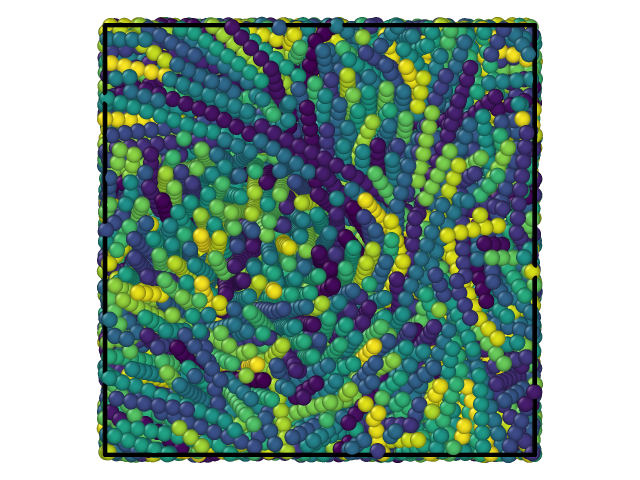
\includegraphics[width=.9\linewidth]{Figures/nun_fr_side}
		\caption{Side View}
		\label{fig:nun_fr_side}
	\end{subfigure}%
	\begin{subfigure}{.5\textwidth}
		\centering
		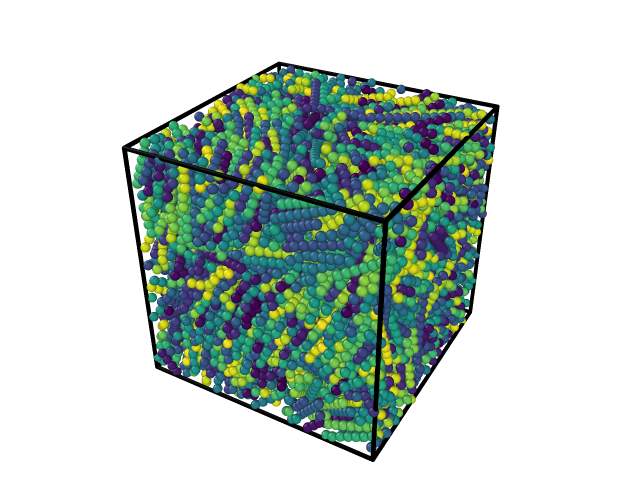
\includegraphics[width=.9\linewidth]{Figures/nun_fr_perspective}
		\caption{Perspective View}
		\label{fig:nun_view_perspective}
	\end{subfigure}
	\caption{The quasi-ordered phase formed by \num{1000} fully flexible nunchucks. Note the local regions of aligned rods, suggesting a nematic-like phase, but also the variation of the director across the sample (between these regions). The length scale of any periodicity in this variation is larger than the simulation box itself.}
	\label{fig:nun_fr_views}
\end{figure} %C:\Users\KitG\Documents\LC_Project\Phase_Structure\Nunchucks\Fixed_Rigidity\stretch500_rigidity5_len15

\begin{figure} [h!]
	\centering
	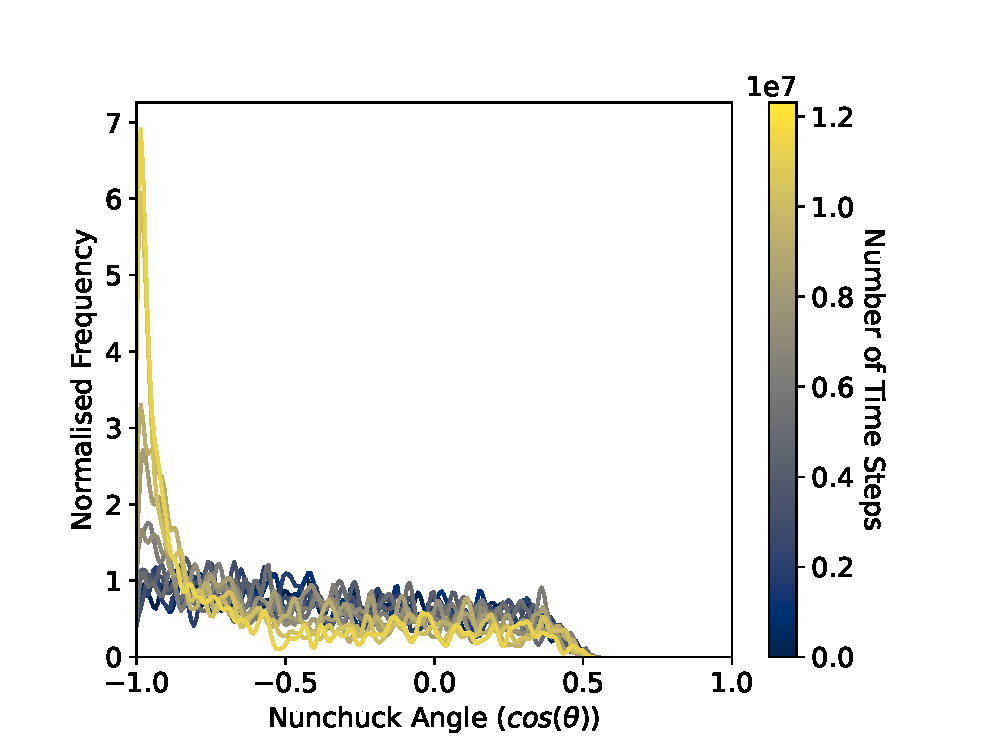
\includegraphics[width=0.7\linewidth]{Figures/nun_fr_angledist}
	\caption{A kernel density estimate plot of the distribution of nunchuck opening angle (between the two rigid arms) over time (as the volume fraction is reduced), where nunchucks are completely flexible. Plotted for a system of \num{1000} particles, with the distribution sampled every \num{1e6} time steps. Note the formation of a preferential angle at late times, corresponding to the formation of an ordered phase at high volume fractions.}
	\label{fig:nun_fr_angledist}
\end{figure}  %C:\Users\KitG\Documents\LC_Project\Phase_Structure\Nunchucks\Fixed_Rigidity 

Consideration of the distribution of nunchuck bond angles (i.e. the opening angle between the two rigid arms) gives further evidence for some ordered phase formation however, with a clear preferential angle forming in Figure \ref{fig:nun_fr_angledist}. We suggest that the length scale over which this director varies is greater than the size of the simulation region, preventing use of the orientational correlation function described in Section \textbf{X} as well. Unfortunately the computational resources required to simulate larger systems was beyond the scope of this project, due to the scaling of the number of particles required to achieve the same volume fractions. However, we suggest similarly quasi-nematic structures may be observed in systems where the nunchuck opening angle is confined to a particular value, particularly if this is below the mean angle in Figure \ref{fig:nun_fr_angledist}.





\subsection{Fixed Angle}

describe quasi-nematic phase seen in both cases
include picture of herringbone-like structure with fixed angle
then go onto orientational order param

\subsection{Orientational Order Parameter}
The suggestion of novel phases in these systems first requires alternative methods to characterise the order of the system; this are typically motivated by the class of symmetry expected here. Given that our system appears to display a degree of orientational order, a length-dependant orientational order parameter is introduced to verify this order is indeed long-ranged (and not simply due to short range steric effects). This also allows the identification of any periodic aspects to the system, as the bend in the nunchucks might be expected to result in the formation of a twisted nematic phase; these would be observed as oscillatory components in the order parameter.

We consider a pair-wise correlation function, where $g(r)$ gives the correlation between the orientation of two particles separated by a distance $r$. 

\textit{equation}

This method is fundamentally limited by the use of a single vector along the molecular axis to define the orientation of the molecule; two vectors (such as along each arm) are required to uniquely specify the orientation of a single molecule. Using the molecule axis alone only accounts for quasi-nematic order; any biaxial or herringbone substructure must be accounted for differently. We therefore also consider orientational correlation functions for the vectors along the bisector of each molecule, and normal to the plane of the nunchuck.



introduce new method to characterise this
detail spherical harmonics approach to calculation in the appendix?

Describe alternative approaches
LOOK INTO BIAXIAL PHASE FURTHER

\section{Dynamic Properties}
Explanation this has only been considered recently, and is much less well understood, as much of the prior simulation work was using MC simulations, which can only predict static properties.
Simplest dynamic property is diffusive coefficient.

Mention simulation complications with periodic bc, and how this was accounted for?
Give power law prediction and my verification of this in dilute systems.
include plots of diffusion coefficient over vol frac for full transition, and rms displacement boxes

Go on to david's theories for dilute and semi-dilute systems? \textit{also review onsager definitions here?}

Explain role in verification of phase formation, particularly for the smectic phase aligned along the y axis.
\section{Conclusion}
Summarise key results from above, and emphasise their importance 
Also give limitations of results obtained, and suggest direction for further work (for each section?)

\section*{Acknowledgements}
I wish to thank my project supervisor (Prof Erika Eiser), and my day-to-day supervisor (Mr Jiaming Yu), as I am very grateful for their continual teaching and advice, and for the initial code provided by Jiaming Yu to run single-stage, rigid-rod simulations. I am also indebted to Prof Daan Frenkel for the kind insights he offered.

%\clearpage
\printbibliography

\begin{appendices}

\section{Onsager Theory} \label{sec:OnsagerAppendix}
A detailed and accessible derivation is provided by Doi and Edwards \cite{Doi1988}, and is not replicated in full here. Briefly summarising their method, the free energy of the system is initially expanded in powers of concentration $\nu$, and higher order terms neglected to give the form:

\begin{equation} \label{eq:OnsagerFreeEnergy}
\mathcal{A}[\Psi(\boldsymbol{u})] = \nu k_{B}T \left[ \ln\nu - 1 + \int d\boldsymbol{u} \Psi(\boldsymbol{u}) \ln \Psi(\boldsymbol{u}) + \frac{1}{2} \int d\boldsymbol{u} \int d\boldsymbol{u^{\prime}} \Psi(\boldsymbol{u}) \Psi(\boldsymbol{u^{\prime}}) \beta(\boldsymbol{u}, \boldsymbol{u^{\prime}})  \right]
\end{equation}

where, for rigid rod-like polymers of diameter $D$ and length $L$, $\beta(\boldsymbol{u}, \boldsymbol{u^{\prime}})$ is given by:

\begin{equation}
\beta(\boldsymbol{u}, \boldsymbol{u^{\prime}}) = 2DL^{2} \left\lvert \boldsymbol{u} \times \boldsymbol{u^{\prime}} \right\rvert
\end{equation} 

This expression may be minimised through the use of a Lagrange multiplier, giving a nonlinear integral equation that cannot be solved linearly. Onsager therefore assumed an equilibrium distribution of the form:

\begin{equation}
\Psi(\boldsymbol{u}) = \frac{\alpha}{4\pi\sinh\alpha} \cosh (\alpha \boldsymbol{u} \cdot \boldsymbol{n})
\end{equation}

for molecule direction $\boldsymbol{u}$, arbitrary unit vector $\boldsymbol{n}$ and order parameter $\alpha$ determined by minimising the free energy. When the concentration exceeds a critical value $\nu^{*}$, a secondary minimum in free energy appears for $\alpha \neq 0$, corresponding to a thermodynamically stable ordered nematic phase. This may not immediately indicate an equilibrium state; indeed Onsager recognised that the free energy may be lowered further by macroscopic phase separation (although we do not expect to observe this in the system sizes considered here). 

Numerical calculation gives $\nu^{*}$, from which the critical volume fraction $\phi^{*}$ may be obtained for rigid rods:

\begin{equation}
\nu^{*} = \frac{16}{\pi D L^{2}}, \qquad \phi^{*} = \nu^{*} \frac{\pi D^{2} L}{4} \simeq 4 \frac{D}{L}
\end{equation}


To derive (\ref{eq:OnsagerFreeEnergy}) that we have assumed it is valid to ignore the third (and higher) Virial coefficients. The reduced third virial coefficient scales as $(D/L)\log(L/D)$, and so is relatively small for the systems considered here. While it should be remembered this may introduce some error in the absolute volume fraction for the phase transition, it does not affect the validity of the phases observed themselves.

It is also acknowledged that this is a poor model experimentally; primarily because physical systems either have much lower aspect ratios or are not truly rigid \cite{Odijk1985}. In this case, the long range Maier\textendash Snape theory \cite{Maier1959} is typically used, with the additional benefit that this also accounts for attractive inter-molecular forces. This produces significantly more accurate estimates of the critical volume fraction and the order parameter at the isotropic\textendash nematic transition \cite{Zannoni1979b}.

\section{Nematic Order Parameter} 
\subsection{Theoretical Outline}\label{sec:OrderParamTheory}
Here I endeavour to outline the motivation for the nematic order parameter used throughout this report, based on the work of Eppenga and Frenkel \cite{Eppenga1984, Frenkel1982}. The nematic phase may be differentiated from the isotropic phase by the formation of cylindrical symmetry, as opposed to the spherical symmetry of the isotropic phase. The deviation from spherical symmetry may be quantified through a set of order parameters \cite{Zannoni1979}. When considering the axially symmetric nematic phase, independent of $\phi$, the distribution function $f(\theta, \phi)$ may be generally expressed in the basis of all even Legendre polynomials $P_{2l}$:

\begin{equation}
f(\theta) = \sum_{l=0}^{\infty} a_{2l} P_{2l}(\cos(\theta))
\end{equation}

where $\theta$ is the angle between the molecular orientation and the axis of symmetry of the system. Note that odd-ordered terms are neglected for nonpolar molecules, as the director may point in either of two antiparallel directions and so all odd Legendre polynomials average to zero \cite{Parsons1979}.

In an isotropic phase, $a_{2l}$ vanishes for all $l>0$, so all angular dependence vanishes. More generally,  quantities $\langle P_{2l}(\cos(\theta)) \rangle$ may be used at the order parameter of the system, with the second order term being referred to as the nematic order parameter. Averaging over a population of $N$ molecules, we can therefore write the nematic order parameter $S_{n}$ as:

\begin{equation}
S_{n} = \frac{1}{N} \left\langle \sum_{i=1}^{N} \left( \frac{3}{2} \cos^{2}(\theta_{i})-\frac{1}{2} \right) \right\rangle
\end{equation}

\subsection{Calculation}\label{sec:OrderParamCalc}
The method given above in Appendix \ref{sec:OrderParamTheory} relies on knowledge of the system-wide nematic director (ie the axis of symmetry of the cylindrical phase), to define $\theta_{i}$. However, this is not always possible in physical systems where such a unique direction is not externally imposed.

Instead, as detailed by Frenkel et al. \cite{Frenkel1985}, we maximise the expression:

\begin{equation} \label{eq:FrenkelNemOrder}
S^{\prime}_{n}(\boldsymbol{\hat{n}^{\prime}}) = \frac{1}{N} \left[ \sum_{i=1}^{N} \left( \frac{3}{2} (\boldsymbol{\hat{n}^{\prime}} \cdot \boldsymbol{\hat{u}_{i}})^{2}-\frac{1}{2} \right) \right]
\end{equation}

where $\hat{u_{i}}$ denotes the orientation of the individual molecular axes in the laboratory frame, and $(\boldsymbol{\hat{n}^{\prime}})$ is the direction of common alignment, known as the director. In the absence of an electric field, the direction of this is arbitrary, and determined in practice by infinitesimal perturbations to the system though spontaneous symmetry breaking \cite{Forster2018}. (\ref{eq:FrenkelNemOrder}) may be further simplified to:

\begin{equation}
S^{\prime}_{n} = \frac{1}{N} \left\langle \boldsymbol{\hat{n}^{\prime}} \cdot \textbf{Q} \cdot \boldsymbol{\hat{n}^{\prime}}  \right\rangle, \qquad where \enspace \textbf{Q}_{i} = \frac{3}{2} \boldsymbol{\hat{u}_{i}}\boldsymbol{\hat{u}_{i}}-\frac{1}{2}\textbf{I}
\end{equation}

The tensor order parameter $\langle \textbf{Q} \rangle$ is a traceless symmetric 2nd-rank tensor, with three eigenvalues $\lambda_{+}, \lambda_{0}, \lambda_{-}$ \cite{Eppenga1984}. We typically take the largest eigenvalue $(\lambda_{+})$ as the nematic order parameter, a good approximation in large N limit.
In practice, we actually calculate the eigenvalues of the related tensor $\textbf{M}$:

\begin{equation}
\textbf{M} =  \frac{1}{N} \sum_{i=1}^{N} \boldsymbol{\hat{u}_{i}}\boldsymbol{\hat{u}_{j}}
\end{equation}

as this shares eigenvectors with $\textbf{Q}$, and has eigenvectors $\mu_{n}$ related to $\lambda_{n}$ by: $\mu_{n} = 2/3 \lambda_{n} + 1/3$.

It is worth noting $\lambda_{+}$ is bound above zero, and so does not reach zero in the isotropic phase as would be expected. It is common to use $S =  -2\lambda_{0}$ when considering such disordered systems, as this fluctuates about an average much closer to zero \cite{Mountain1977}. I have not done so in the results presented here, to give continuity in the order parameter over the transition (wherein lies the focus of this report), however this has meant that the average order parameter in the isotropic phase is slightly above zero.


\section{Code?}

\end{appendices}

\end{document}


%%%%%%%%%%%%%%%%%%%%%%%%%%%%%%%%%%%%%%%%%
% Wenneker Article
% LaTeX Template
% Version 2.0 (28/2/17)
%
% This template was downloaded from:
% http://www.LaTeXTemplates.com
%
% Authors:
% Vel (vel@LaTeXTemplates.com)
% Frits Wenneker
%
% License:
% CC BY-NC-SA 3.0 (http://creativecommons.org/licenses/by-nc-sa/3.0/)
%
%%%%%%%%%%%%%%%%%%%%%%%%%%%%%%%%%%%%%%%%%
